\documentclass[12pt]{article}

% --- Core math + proof tools ---
\usepackage{amsmath, amssymb, amsthm}

% --- Lists and spacing ---
\usepackage{enumitem}
\setlist[enumerate,1]{label=\textbf{(\alph*)}, leftmargin=2em, itemsep=0.25em}
\setlist[itemize]{leftmargin=1.5em, itemsep=0.25em}
\setlength{\parskip}{0.35em}
\setlength{\parindent}{0pt}

% --- Page geometry + header/footer ---
\usepackage{geometry}
\usepackage{multicol} % for problem 5
\geometry{margin=1in}
\usepackage{csquotes} % to use blockquotes
\usepackage{graphicx} % for figures
\graphicspath{{images/}} % tells LaTeX to look in the “images” folder

\usepackage{fancyhdr}
\pagestyle{fancy}
\fancyhf{}
\rhead{MATH 421 — 003, Fall 2025}
\lhead{Homework 7}
\cfoot{\thepage}
\renewcommand{\headrulewidth}{0.4pt}

% --- Links (nice for references, stays subtle) ---
\usepackage[hidelinks]{hyperref}

% --- Title info ---
\title{Homework 7}
\author{Alejandro De La Torre \\ MATH 421 — The Theory of Single Variable Calculus \\ Section 003 \\ Instructor: Grace Work}
\date{October 2025}

% --- (Optional) proof environments you might want ---
\newtheorem*{claim}{Claim}
\newtheorem*{lemma}{Lemma}
\newtheorem*{remark}{Remark}

% --- Convenience: a Problem header command ---
\newcommand{\problem}[2][]{%
  \vspace{0.5em}
  \hrule\vspace{0.4em}
  \textbf{Problem #2}\if\relax\detokenize{#1}\relax\else\; \textit{(#1)}\fi
  \vspace{0.25em}\hrule\vspace{0.8em}
}

% --- Convenience: an ignore command to comment out blocks ---
\newcommand{\ignore}[1]{}


\begin{document}
\maketitle

% ------------------ collaboration + sources ------------------
\section*{Collaboration Statement}
% (List any classmates you collaborated with here, or write ``I worked alone'' if you did not collaborate with anyone.)

\bigskip

% ------------------ problem 1 ------------------
\problem[Ross Chapter 2 11.4]{1}
Repeat Exercise 11.2 for the sequences: \\
$w_n = -(2)^n$, $x_n= 5 ^{(-1)^{n}}$, $y_n=1+(-1)^n$, $z_n=n \cos(\frac{n \pi}{4})$.\\
\vspace{0.05cm}

\textit{Question 11.2 asks you to do the following for each sequence}:

\begin{enumerate}[label=(\alph*)]
    \item For each sequence, give an example of a monotone subsequence.
    \item For each sequence, give its set of subsequential limits.
    \item For each sequence, give its $\lim \sup$ and $\lim \inf$.
    \item Which of the sequences converges? diverges to $+\infty$? diverges to $-\infty$?
    \item Which of the sequences is bounded?
\end{enumerate}
\vspace{0.75em}

\textbf{Discussion.} \\
%(Very brief plan / key ideas.)
\vspace{0.25em}

\textbf{Proof.}\\
% (Your proof goes here.)
\qed

% ------------------ problem 2 ------------------
\problem[Ross Chapter 2 11.8]{2}
Use Definition 10.6 and Exercise 5.4 to prove $\lim \inf s_n = - \lim \sup (-s_n)$ for every sequence ($s_n$).
\\
\vspace{0.75em}
\textbf{Discussion.} \\
\textbf{10.6 Definition}:\\
Let ($s_n$) be a sequence in $\mathbb{R}$. We define: \\
\[
\lim \sup s_n = \lim_{N \to \infty} \sup \{ s_n : n \geq N \}
\]
and
\[
\lim \inf s_n = \lim_{N \to \infty} \inf \{ s_n : n \geq N \}
\]
\\
\textbf{5.4 Exercise}:\\
Let $S$ be a nonempty subset $\mathbb{R}$, and let $-S = { -s : s \in S }$. Prove $\inf S = -\sup(-S)$. \textit{Hint: For the case $-\infty < \inf S$, simply state that this was proved in Exercise 4.9}.

\vspace{0.25em}
\textbf{Proof.}\\
% (Your proof goes here.)
\qed

% ------------------ problem 3 ------------------
\problem[Ross Chapter 2 11.10]{3}
Let ($s_n$) be the sequence of numbers in Fig. 11.2 listed in the indicated
order.
\begin{enumerate}[label=(\alph*)]
    \item Find the set $S$ of subsequential limits of ($s_n$).
    \item Determine $\lim \sup s_n$ and $\lim \inf s_n$.
\end{enumerate}

\begin{center}
    \begin{figure}[h!]
        \centering
        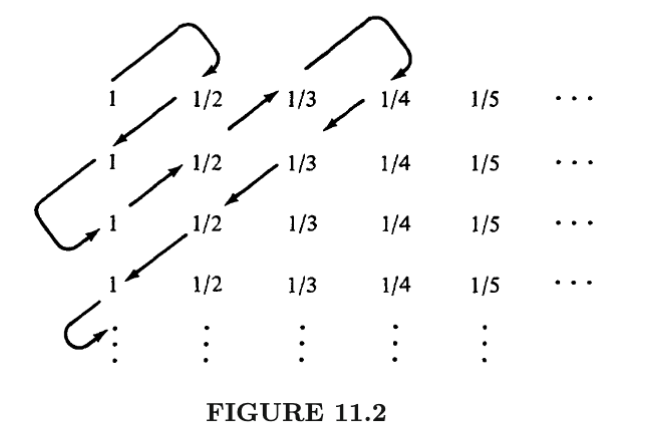
\includegraphics[width=0.7\textwidth]{figure_11_2.png}
        \label{fig:subseq-illustration}
    \end{figure}
\end{center}

\vspace{0.75em}
\textbf{Discussion.} \\
%(Very brief plan / key ideas.)
\vspace{0.25em}
\textbf{Proof.}\\
% (Your proof goes here.)
\qed

% ------------------ problem 4------------------
\problem[Ross Chapter 2 12.2]{4}
Prove $\lim \sup | s_n | = 0$ if and only if $\lim s_n = 0$.
\vspace{0.75em}
\textbf{Discussion.} \\
%(Very brief plan / key ideas.)
\vspace{0.25em}
\textbf{Proof.}\\
% (Your proof goes here.)
\qed


% ------------------ problem 5 ------------------
\problem[Ross Chapter 2 12.3]{5}
Let ($s_n$) and ($t_n$) be the following sequences that repeat in cycles of
four:
\[
    (s_n) = (0, 1, 2, 1, 0, 1, 2, 1, 0, 1, 2, 1, 0, 1, 2, 1, 0, . . .) 
\]
\[
    (t_n) = (2, 1, 1, 0, 2, 1, 1, 0, 2, 1, 1, 0, 2, 1, 1, 0, 2, . . .)
\]
Find
\begin{multicols}{2}
\begin{enumerate}[label=(\alph*)]
    \item $\liminf s_n + \liminf t_n$
    \item $\liminf (s_n + t_n)$
    \item $\liminf s_n + \limsup t_n$
    \item $\limsup (s_n + t_n)$
    \item $\limsup s_n + \limsup t_n$
    \item $\liminf (s_n t_n)$
    \item $\limsup (s_n t_n)$
\end{enumerate}
\end{multicols}

\vspace{0.75em}
\textbf{Discussion.} \\
%(Very brief plan / key ideas.)
\vspace{0.25em}
\textbf{Proof.}\\
% (Your proof goes here.)
\qed

% ------------------ problem 6 ------------------
\problem[Ross Chapter 2 12.10]{6}
Prove ($s_n$) is bounded if and only if $\lim \sup | s_n | < +\infty$.\\
\vspace{0.75em}
\textbf{Discussion.} \\
%(Very brief plan / key ideas.)
\vspace{0.25em}
\textbf{Proof.}\\
% (Your proof goes here.)
\qed
\end{document}